\subsubsection{Implicit Assertions} \label{Sec:implicitAssertions}
We gather all the statements that explicitly affect the computations relevant to a given DOM-based assertion. While assertions inferred from such statements are inherently important, we further need to consider entities that are implicitly influenced by the checked DOM element in the manually-written test suite. For this purpose we apply a dynamic forward slice on the statements collected from a backward slice of a DOM-based assertion.
%\begin{mydef}[Forward Slicing]
%\label{def:forwardSlicing} 
%A forward slice of a program with respect to a statement $st$ at program point $p$ and set of program variables $V$ consists of all statements and predicates in the program that are affected by the value of variables in $V$ at $p$.
%\end{mydef}
A forward slice with respect to a statement $st$,
indicates how subsequently an operand at $st$ is being used. This can help the tester to ensure that $st$ establishes the expected outcome of the computations assumed by later statements. 
%Given the importance of statements involved in code-level computations of a DOM-based assertion, using forward slice is useful to check that there are no unforeseen effects on the application's behavior by a modification to such statements. 

\begin{figure}[!t]
  \centering
  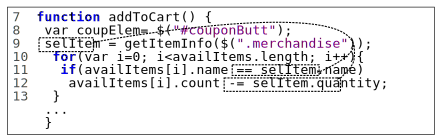
\includegraphics[width=1\hsize]{fig/forwardSlicingExample}
   \vspace{-0.2in} 
  \mycaption{Forward Slicing to obtain implicit assertions.}
  \label{Fig:forwardSlicingExample}
 % \vspace{-0.1in} 
\end{figure}

Dynamic forward slice is performed on the subset of code statements which is previously instrumented as explained in \secref{domToCode}. 
\textsc{GetFWSlice} in line 17 of the algorithm computes forward slice on the variable operands of a statement in the backward slice.
The process of forward slicing is similar to the backward slicing technique discussed earlier (\secref{domToCode}). The slicing criterion of the forward slice module is either a variable, object's property, or an accessed DOM property extracted from the statements in a backward slice segments of the code. The accessible entities (\textsc{Accessibles} in line 24), which have been set within the collected forward slice statements establish the implicit assertions.
$implicitAsstn$ in line 24 of \algref{algorithm} contains the inferred implicit assertions.
\figref{forwardSlicingExample} shows the relevant parts of the code obtained by performing forward slicing on the running example. 
As shown in the figure, the properties of object \code{selItem} are set in line 16, that is recorded during the backward slice process. Given line 16 as the forward slice criteria, we mark \code{availItems.count} (line 19) as an implicit assertion.        